\documentclass[authordate, empirical]{jote-new-article}

\usepackage{caption}

\usepackage{tabularx}

\usepackage{graphicx}

\usepackage{hyperref}

\usepackage[backend=biber,style=apa]{biblatex}

\addbibresource{bibliography.bib}

\jotetitle{Three Persistent Myths about Open Science}
\keywordsabstract{open science, diversity, data sharing, preregistration, meta-science}
\abstracttext{Knowledge and implementation of open science principles and behaviors remains uneven across the sciences, despite over 10 years of intensive education and advocacy. One reason for the slow and uneven progress of the open science movement is a set of closely held myths about the implications of open science practices, bolstered by recurring objections and arguments that have long been addressed. This paper covers three of these major recurring myths: 1) that open science conflicts with prioritizing diversity, 2) that “open data” is a binary choice between fully open and accessible and completely closed off, and 3) that preregistration is only appropriate for certain types of research designs. Putting these myths to rest is necessary as we work towards improving our scientific practice.}
\runningauthor{Syed}
\jname{Journal of Trial \& Error}
\jyear{2024}
\paperdoi{10.36850/mr11}
\paperreceived{September 12, 2023}
\author[1]{\mbox{Moin Syed\orcid{0000-0003-4759-3555}}}
\affil[1]{University of Minnesota}
\corremail{\href{mailto:moin@umn.edu}{moin@umn.edu}}
\corraddress{University of Minnesota}
\runningauthor{Syed}
\paperaccepted{January 25, 2024}
\paperpublished{March 31, 2024}
\paperpublisheddate{2024-03-31}
\jwebsite{https://journal.trialanderror.org}

\begin{filecontents}{bibliography.bib}
	@article{Arnett2008,
    title       = {The neglected 95\%: {W}hy {A}merican psychology needs to become less {A}merican},
    author      = {Arnett, J. J.},
    number      = {7},
    volume      = {63},
    url         = {https://doi.org/10.1037/0003-066X.63.7.602},
    doi         = {10.1037/0003-066X.63.7.602},
    date        = {2008},
    pages       = {602--614},
    journal     = {American Psychologist}
}


@article{Askarov2023,
    title       = {Selective and (mis)leading economics journals: {M}eta-research evidence},
    author      = {Askarov, Z. and Doucouliagos, A. and Doucouliagos, H. and Stanley, T. D.},
    url         = {https://doi.org/10.1111/joes.12598},
    doi         = {10.1111/joes.12598},
    date        = {2023},
    pages       = {1--26},
    journal     = {Journal of Economic Surveys}
}


@article{Azevedo2019,
    title       = {Introducing a Framework for Open and Reproducible Research Training ({FORRT})},
    journal = {{OSF} Preprints},
    author      = {Azevedo, F. and Parsons, S. and Micheli, L. and Strand, J. and Rinke, E. and Guay, S. and Elsherif, M. and Quinn, K. and Wagge, J. R. and Steltenpohl, C. and Kalandadze, T. and Vasilev, M. and de Oliveira, C. F. and Aczel, B. and Miranda, J. and Galang, C. M. and Baker, B. J. and Pennington, C. R. and Marques, T. and {FORRT}},
    url         = {https://doi.org/10.31219/osf.io/bnh7p},
    doi         = {10.31219/osf.io/bnh7p},
    date        = {2019-12-13}
}


@article{Bergmann2023,
    title       = {The buffet approach to open science},
    author      = {Bergmann, C.},
    url         = {https://cogtales.wordpress.com/2023/04/16/the-buffet-approach-to-open-science/},
    date        = {2023-04-16},
    journal     = {CogTales}
}


@article{Bahlai2019,
    title       = {Open science isn't always open to all scientists},
    author      = {Bahlai, C. and Bartlett, L. and Burgio, K. and Fournier, A. and Keiser, C. and Poisot, T. and Whitney, K.},
    number      = {2},
    volume      = {107},
    url         = {https://doi.org/10.1511/2019.107.2.78},
    doi         = {10.1511/2019.107.2.78},
    date        = {2019},
    pages       = {78},
    journal     = {American Scientist}
}


@article{Baker2016,
    title       = {1,500 scientists lift the lid on reproducibility},
    author      = {Baker, M.},
    volume      = {533},
    url         = {https://doi.org/10.1038/533452a},
    doi         = {10.1038/533452a},
    date        = {2016},
    eid         = {452-454},
    journal     = {Nature}
}


@article{Baumeister2007,
    title       = {Psychology as the science of self-reports and finger movements: {W}hatever happened to actual behavior?},
    author      = {Baumeister, R. F. and Vohs, K. D. and Funder, D. C.},
    number      = {4},
    volume      = {2},
    url         = {https://doi.org/10.1111/j.1745-6916.2007.00051.x},
    doi         = {10.1111/j.1745-6916.2007.00051.x},
    date        = {2007},
    pages       = {396--403},
    journal     = {Perspectives on Psychological Science}
}


@article{Beer2023,
    title       = {Hits and misses in the last decade of open science: {R}esearchers from different subfields and career stages offer personal reflections and suggestions},
    author      = {Beer, J. and Eastwick, P. and Goh, J. X.},
    volume      = {18},
    url         = {https://doi.org/10.32872/spb.9681},
    doi         = {10.32872/spb.9681},
    date        = {2023},
    pages       = {1--23},
    journal     = {Social Psychological Bulletin}
}


@article{Bem2011,
    title       = {Feeling the future: {E}xperimental evidence for anomalous retroactive influences on cognition and affect},
    author      = {Bem, D. J.},
    number      = {3},
    volume      = {100},
    url         = {https://doi.org/10.1037/a0021524},
    doi         = {10.1037/a0021524},
    date        = {2011},
    pages       = {407--425},
    journal     = {Journal of Personality and Social Psychology}
}


@article{Brembs2018,
    title       = {Prestigious science journals struggle to reach even average reliability},
    author      = {Brembs, B.},
    volume      = {12},
    url         = {https://doi.org/10.3389/fnhum.2018.00037},
    doi         = {10.3389/fnhum.2018.00037},
    date        = {2018},
    pages       = {37},
    journal     = {Frontiers in Human Neuroscience}
}


@article{Causadias2021,
    title       = {The importance of research about research on culture: {A} call for meta-research on culture},
    author      = {Causadias, J. M. and Korous, K. M. and Cahill, K. M. and Rea-Sandin, G.},
    number      = {1},
    volume      = {29},
    url         = {https://doi.org/10.1037/cdp0000516},
    doi         = {10.1037/cdp0000516},
    date        = {2021},
    pages       = {85--95},
    journal     = {Cultural Diversity and Ethnic Minority Psychology}
}


@book{Chambers2017,
    title       = {The seven deadly sins of psychology: {A} manifesto for reforming the culture of scientific practice},
    author      = {Chambers, C. D.},
    publisher   = {Princeton University Press},
    date        = {2017}
}


@article{Chambers2020,
    title       = {Verification Reports: {A} new article type at {C}ortex},
    author      = {Chambers, C. D.},
    volume      = {129},
    url         = {https://doi.org/10.1016/j.cortex.2020.04.020},
    doi         = {10.1016/j.cortex.2020.04.020},
    date        = {2020},
    pages       = {1-- 3},
    journal     = {Cortex}
}


@article{Chambers2021,
    title       = {The past, present and future of Registered Reports},
    author      = {Chambers, C. D. and Tzavella, L.},
    volume      = {6},
    url         = {https://doi.org/10.1038/s41562-021-01193-7},
    doi         = {10.1038/s41562-021-01193-7},
    date        = {2021},
    pages       = {29--42},
    journal     = {Nature Human Behaviour}
}


@article{Cialdini2009,
    title       = {We have to break up},
    author      = {Cialdini, R. B.},
    number      = {1},
    volume      = {4},
    url         = {https://doi.org/10.1111/j.1745-6924.2009.01091.x},
    doi         = {10.1111/j.1745-6924.2009.01091.x},
    date        = {2009},
    pages       = {5--6},
    journal     = {Perspectives on Psychological Science}
}


@article{Claesen2021,
    title       = {Comparing dream to reality: {A}n assessment of adherence of the first generation of preregistered studies},
    author      = {Claesen, A. and Gomes, S. and Tuerlinckx, F. and Vanpaemel, W.},
    number      = {10},
    volume      = {8},
    url         = {https://doi.org/10.1098/rsos.211037},
    doi         = {10.1098/rsos.211037},
    date        = {2021},
    pages       = {211037},
    journal     = {Royal Society Open Science}
}


@article{Draper2022,
    title       = {Publishing child development research from around the world: {A}n unfair playing field resulting in most of the world's child population under-represented in research},
    author      = {Draper, C. E. and Barnett, L. M. and Cook, C. J. and Cuartas, J. A. and Howard, S. J. and McCoy, D. C. and Merkley, R. and Molano, A. and Maldonado-Carreño, C. and Obradović, J. and Scerif, G. and Valentini, N. C. and Venetsanou, F. and Yousafzai, A. K.},
    number      = {6},
    volume      = {32},
    url         = {https://doi.org/10.1002/icd.2375},
    doi         = {10.1002/icd.2375},
    date        = {2022},
    journal     = {Infant and Child Development},
    eid         = {Article e2375}
}


@article{Elsherif2022,
    title       = {Bridging neurodiversity and open scholarship: {H}ow shared values can guide best practices for research integrity},
    author      = {Elsherif, M. M. and Middleton, S. L. and Phan, J. M. and Azevedo, F. and Iley, B. J. and Grose-Hodge, M. and Tyler, S. L. and Kapp, S. K. and Gourdon-Kanhukamwe, A. and Grafton-Clarke, D. and Yeung, S. K. and Shaw, J. J. and Hartmann, H. and Dokovova, M.},
    url         = {https://doi.org/10.31222/osf.io/k7a9p.},
    doi         = {10.31222/osf.io/k7a9p.},
    date        = {2022-06-20}
}


@article{Errington2021,
    title       = {Challenges for assessing replicability in preclinical cancer biology},
    author      = {Errington, T. M. and Denis, A. and Perfito, N. and Iorns, E. and A, Nosek B.},
    volume      = {10},
    eid         = {Article e67995},
    url         = {https://doi.org/10.7554/eLife.67995},
    doi         = {10.7554/eLife.67995},
    date        = {2021},
    journal     = {eLife}
}


@article{Farnham2017,
    title       = {Early career researchers want {O}pen {S}cience},
    author      = {Farnham, A. and Kurz, C. and Öztürk, M. A. and Solbiati, M. and Myllyntaus, O. and Meekes, J. and Pham, T. M. and Paz, C. and Langiewicz, M. and Andrews, S. and Kanninen, L. and Agbemabiese, C. and Guler, A. T. and Durieux, J. and Jasim, S. and Viessmann, O. and Frattini, S. and Yembergenova, D. and Benito, C. M. and Hettne, K.},
    number      = {1},
    volume      = {18},
    url         = {https://doi.org/10.1186/s13059-017-1351-7},
    doi         = {10.1186/s13059-017-1351-7},
    date        = {2017},
    eid         = {Article 221},
    journal     = {Genome Biology}
}


@article{Field2021,
    title       = {Qualitative open science--pain points and perspectives},
    author      = {Field, S. M. and van Ravenzwaaij, D. and Pittelkow, M. M. and Hoek, J. M. and Derksen, M.},
    url         = {https://osf.io/e3cq4/},
    date        = {2021},
    journal     = {OSF Preprints}
}


@article{Fleming2021,
    title       = {Open accessibility in education research: {E}nhancing the credibility, equity, impact, and efficiency of research},
    author      = {Fleming, J. I. and Wilson, S. E. and Hart, S. A. and Therrien, W. J. and Cook, B. G.},
    number      = {2},
    volume      = {56},
    url         = {https://doi.org/10.1080/00461520.2021.1897593},
    doi         = {10.1080/00461520.2021.1897593},
    date        = {2021},
    pages       = {110--121},
    journal     = {Educational Psychologist}
}


@article{FoxTree2022,
    title       = {The inequitable burden of open science},
    author      = {Fox Tree, J. and Lleras, A. and Thomas, A. and Watson, D.},
    url         = {https://featuredcontent.psychonomic.org/the-inequitable-burden-of-open-science/},
    date        = {2022-08-30}
}


@article{Fraser2018,
    title       = {Questionable research practices in ecology and evolution},
    author      = {Fraser, H. and Parker, T. and Nakagawa, S. and Barnett, A. and Fidler, F.},
    number      = {7},
    volume      = {13},
    url         = {https://doi.org/10.1371/journal.pone.0200303},
    doi         = {10.1371/journal.pone.0200303},
    date        = {2018},
    journal     = {PLOS ONE},
    eid         = {Article e0200303}
}


@article{Fuentes2022,
    title       = {Open science: {F}riend, foe, or both to an antiracist psychology?},
    author      = {Fuentes, M. A. and Zelaya, D. G. and Delgado-Romero, E. A. and Butt, M.},
    number      = {5},
    volume      = {130},
    url         = {https://doi.org/10.1037/rev0000386},
    doi         = {10.1037/rev0000386},
    date        = {2022},
    pages       = {1351--1359},
    journal     = {Psychological Review}
}


@article{Gabelica2022,
    title       = {Many researchers were not compliant with their published data sharing statement: mixed-methods study},
    author      = {Gabelica, M. and Bojčić, R. and Puljak, L.},
    volume      = {150},
    url         = {https://doi.org/10.1016/j.jclinepi.2022.05.019},
    doi         = {10.1016/j.jclinepi.2022.05.019},
    date        = {2022},
    pages       = {33--41},
    journal     = {Journal of Clinical Epidemiology}
}


@inbook{Gilmore2016,
    title       = {Curating identifiable data for sharing: {T}he {D}atabrary project},
    author      = {Gilmore, R. O. and Adolph, K. E. and Millman, D. S.},
    url         = {https://doi.org/10.1109/NYSDS.2016.7747817},
    doi         = {10.1109/NYSDS.2016.7747817},
    publisher   = {IEEE},
    date        = {2016-08},
    pages       = {1--6},
    booktitle     = {2016 {New York Scientific Data Summit (NYSDS)}}
}


@article{Graham1992,
    title       = {"Most of the subjects were {W}hite and middle class": {T}rends in published research on {A}frican {A}mericans in selected {APA} journals, 1970--1989},
    author      = {Graham, S.},
    number      = {5},
    volume      = {47},
    url         = {https://doi.org/10.1037/0003-066X.47.5.629},
    doi         = {10.1037/0003-066X.47.5.629},
    date        = {1992},
    pages       = {629--639},
    journal     = {American Psychologist}
}


@article{Green2022,
    title       = {A perspective on enhancing representative samples in developmental human neuroscience: {C}onnecting science to society},
    author      = {Green, K. H. and Van De Groep, I. H. and Te Brinke, L. W. and van der Cruijsen, R. and van Rossenberg, F. and El Marroun, H.},
    volume      = {16},
    eid         = {Article 981657},
    url         = {https://www.frontiersin.org/articles/10.3389/fnint.2022.981657},
    date        = {2022},
    journal     = {Frontiers in Integrative Neuroscience}
}


@article{Grzanka2021,
    title       = {An argument for bad psychology: {D}isciplinary disruption, public engagement, and social transformation},
    author      = {Grzanka, P. R. and Cole, E. R.},
    number      = {8},
    volume      = {76},
    url         = {https://doi.org/10.1037/amp0000853},
    doi         = {10.1037/amp0000853},
    date        = {2021},
    pages       = {1334--1345},
    journal     = {American Psychologist}
}


@book{Guthrie1976,
    title       = {The rat was white: {A} historical view of psychology},
    author      = {Guthrie, R. V.},
    publisher   = {Allyn \& Bacon},
    date        = {1976}
}


@article{Hall2001,
    title       = {In search of cultural diversity: {R}ecent literature in cross-cultural and ethnic minority psychology},
    author      = {Hall, G. C. N. and Maramba, G. G.},
    number      = {1},
    volume      = {7},
    url         = {https://doi.org/10.1037/1099-9809.7.1.12},
    doi         = {10.1037/1099-9809.7.1.12},
    date        = {2001},
    pages       = {12--26},
    journal     = {Cultural Diversity and Ethnic Minority Psychology}
}


@article{Hart2020,
    title       = {{LD}base},
    author      = {Hart, S. A. and Schatschneider, C. and Reynolds, T. R. and Calvo, F. E. and Brown, B. J. and Arsenault, B. and Hall, M. R. K. and van Dijk, W. and Edwards, A. A. and Shero, J. A. and Smart, R. and Phillips, J. S.},
    url         = {http://doi.org/10.33009/ldbase.},
    doi         = {10.33009/ldbase.},
    date        = {2020}
}


@article{Hartmann2013,
    title       = {In Search of Cultural Diversity, Revisited: {R}ecent publication trends in cross-cultural and ethnic minority psychology},
    author      = {Hartmann, W. E. and Kim, E. S. and Kim, J. H. J. and Nguyen, T. U. and Wendt, D. C. and Nagata, D. K. and Gone, J. P.},
    number      = {3},
    volume      = {17},
    url         = {https://doi.org/10.1037/a0032260},
    doi         = {10.1037/a0032260},
    date        = {2013},
    pages       = {243--254},
    journal     = {Review of General Psychology}
}


@article{Haven2019,
    title       = {Preregistering qualitative research},
    author      = {Haven, T. and Van Grootel and L, Dr},
    number      = {3},
    volume      = {26},
    url         = {https://doi.org/10.1080/08989621.2019.1580147},
    doi         = {10.1080/08989621.2019.1580147},
    date        = {2019},
    pages       = {229--244},
    journal     = {Accountability in Research}
}


@article{Henrich2010,
    title       = {The weirdest people in the world?},
    author      = {Henrich, J. and Heine, S. J. and Norenzayan, A.},
    number      = {2--3},
    volume      = {33},
    url         = {https://doi.org/10.1017/S0140525X0999152X},
    doi         = {10.1017/S0140525X0999152X},
    date        = {2010},
    pages       = {61--83},
    journal     = {Behavioral and Brain Sciences}
}


@article{Humphreys2021,
    title       = {Integrating qualitative methods and open science: {F}ive principles for more trustworthy research},
    author      = {Humphreys, L. and Lewis, N. A. and Sender, K. and Won, A. S.},
    number      = {5},
    volume      = {71},
    url         = {https://doi.org/10.1093/joc/jqab026},
    doi         = {10.1093/joc/jqab026},
    date        = {2021},
    pages       = {855--874},
    journal     = {Journal of Communication}
}


@article{Kidwell2016,
    title       = {Badges to Acknowledge Open Practices: {A} simple, low-cost, effective method for increasing transparency},
    author      = {Kidwell, M. C. and Lazarević, L. B. and Baranski, E. and Hardwicke, T. E. and Piechowski, S. and Falkenberg, L.-S. and Kennett, C. and Slowik, A. and Sonnleitner, C. and Hess-Holden, C. and Errington, T. M. and Fiedler, S. and Nosek, B. A.},
    number      = {5},
    volume      = {14},
    url         = {https://doi.org/10.1371/journal.pbio.1002456},
    doi         = {10.1371/journal.pbio.1002456},
    date        = {2016},
    eid         = {Article 1002456},
    journal     = {PLOS Biology}
}


@article{Knöchelmann2019,
    title       = {Open {S}cience in the Humanities, or: {O}pen Humanities?},
    author      = {Knöchelmann, M.},
    number      = {4},
    volume      = {7},
    url         = {https://doi.org/10.3390/publications7040065},
    doi         = {10.3390/publications7040065},
    date        = {2019},
    pages       = {65},
    journal     = {Publications}
}


@article{Lakens2019,
    title       = {The value of preregistration for psychological science: {A} conceptual analysis},
    author      = {Lakens, D.},
    url         = {https://doi.org/10.31234/osf.io/jbh4w},
    doi         = {10.31234/osf.io/jbh4w},
    date        = {2019},
    journal     = {PsyArXiv}
}


@article{LeBel2011,
    title       = {Fearing the future of empirical psychology: {B}em's (2011) evidence of psi as a case study of deficiencies in modal research practice},
    author      = {LeBel, E. P. and Peters, K. R.},
    number      = {4},
    volume      = {15},
    url         = {https://doi.org/10.1037/a0025172},
    doi         = {10.1037/a0025172},
    date        = {2011},
    pages       = {371--379},
    journal     = {Review of General Psychology}
}


@article{Ledgerwood2022,
    title       = {The pandemic as a portal: {R}eimagining psychological science as truly open and inclusive.},
    author      = {Ledgerwood, A. and Hudson, S. K. T. J. and Lewis Jr, N. A. and Maddox, K. B. and Pickett, C. L. and Remedios, J. D. and Cheryan, S. and Diekman, A. B. and Dutra, N. B. and Goh, J. X. and Goodwin, S. A. and Munakata, Y. and Navarro, D. J. and Onyeador, I. N. and Srivastava, S. and Wilkins, C. L.},
    number      = {4},
    volume      = {17},
    url         = {https://doi.org/10.1177/17456916211036654},
    doi         = {10.1177/17456916211036654},
    date        = {2022},
    pages       = {937--959},
    journal     = {Perspectives on Psychological Science}
}


@article{Lee2017,
    title       = {Editorial},
    author      = {Lee, R. M.},
    number      = {3},
    volume      = {23},
    url         = {https://doi.org/10.1037/cdp0000172},
    doi         = {10.1037/cdp0000172},
    date        = {2017},
    pages       = {311},
    journal     = {Cultural Diversity and Ethnic Minority Psychology}
}


@article{Lewis2017,
    title       = {Reflections on {SIPS} (guest post by {N}eil {Lewis, Jr.})}, 
    journal     = {The Hardest Science},
    author      = {Lewis, N.},
    url         = {https://thehardestscience.com/2017/08/11/reflections-on-sips-guest-post-by-neil-lewis-jr/},
    date        = {2017-08-11}
}


@article{Lin2022,
    title       = {Global diversity of authors, editors, and journal ownership across subdisciplines of psychology: {C}urrent state and policy implications},
    author      = {Lin, Z. and Li, N.},
    number      = {2},
    volume      = {18},
    url         = {https://doi.org/10.1177/17456916221091831},
    doi         = {10.1177/17456916221091831},
    date        = {2022},
    pages       = {358--377},
    journal     = {Perspectives on Psychological Science}
}


@article{Lui2022,
    title       = {Open science and multicultural research: {S}ome data, considerations, and recommendations},
    author      = {Lui, P. P. and Gobrial, S. and Pham, S. and Giadolor, W. and Adams, N. and Rollock, D.},
    number      = {4},
    volume      = {28},
    url         = {https://doi.org/10.1037/cdp0000541},
    doi         = {10.1037/cdp0000541},
    date        = {2022},
    pages       = {567--586},
    journal     = {Cultural Diversity and Ethnic Minority Psychology}
}


@article{MacEachern2019,
    title       = {Preregistration of modeling exercises may not be useful},
    author      = {MacEachern, S. N. and Van Zandt, T.},
    number      = {3},
    volume      = {2},
    url         = {https://doi.org/10.1007/s42113-019-00038-x},
    doi         = {10.1007/s42113-019-00038-x},
    date        = {2019},
    pages       = {179--182},
    journal     = {Computational Brain \& Behavior}
}


@article{McDermott2022,
    title       = {Breaking free: {H}ow preregistration hurts scholars and science},
    author      = {McDermott, R.},
    number      = {1},
    volume      = {41},
    url         = {https://doi.org/10.1017/pls.2022.4},
    doi         = {10.1017/pls.2022.4},
    date        = {2022},
    pages       = {55--59},
    journal     = {Politics and the Life Sciences}
}


@article{Meyer2018,
    title       = {Practical tips for ethical data sharing},
    author      = {Meyer, M. N.},
    number      = {1},
    volume      = {1},
    url         = {https://doi.org/10.1177/2515245917747656},
    doi         = {10.1177/2515245917747656},
    date        = {2018},
    pages       = {131--144},
    journal     = {Advances in Methods and Practices in Psychological Science}
}


@article{Miyakawa2020,
    title       = {No raw data, no science: another possible source of the reproducibility crisis},
    author      = {Miyakawa, T.},
    number      = {1},
    volume      = {13},
    url         = {https://doi.org/10.1186/s13041-020-0552-2},
    doi         = {10.1186/s13041-020-0552-2},
    date        = {2020},
    pages       = {1--6},
    journal     = {Molecular Brain}
}


@article{Moreau2022,
    title       = {Conducting a meta-analysis in the age of open science: {T}ools, tips, and practical recommendations},
    author      = {Moreau, D. and Gamble, B.},
    number      = {3},
    volume      = {27},
    url         = {https://doi.org/10.1037/met0000351},
    doi         = {10.1037/met0000351},
    date        = {2022},
    pages       = {426--432},
    journal     = {Psychological Methods}
}


@article{Moriguchi2022,
    title       = {Beyond bias to {W}estern participants, authors, and editors in developmental science}, 
    journal = {Infant and Child Development}, 
    volume={31},
    issue={1},
    author      = {Moriguchi, Y.},
    url         = {https://doi.org/10.1002/icd.2256},
    doi         = {10.1002/icd.2256},
    date        = {2022},
    eid         = {Article e2256}
}


@article{Moshontz2021,
    title       = {A guide to posting and managing preprints},
    author      = {Moshontz, H. and Binion, G. E. and Walton, H. and Brown, B. T. and Syed, M.},
    number      = {2},
    volume      = {4},
    date        = {2021},
    pages       = {1--11},
    journal     = {Advances in Methods and Practices in Psychological Science}
}


@article{Moshontz2018,
    title       = {The {P}sychological {S}cience {A}ccelerator: {A}dvancing psychology through a distributed collaborative network},
    author      = {Moshontz, H. and Campbell, L. and Ebersole, C. R. and IJzerman, H. and Urry, H. L. and Forscher, P. S. and Grahe, J. E. and McCarthy, R. J. and Musser, E. D. and Antfolk, J. and Castille, C. M. and Evans, T. R. and Fiedler, S. and Flake, J. K. and Forero, D. A. and Janssen, S. M. J. and Keene, J. R. and Protzko, J. and Aczel, B. and Chartier, C. R.},
    number      = {4},
    volume      = {1},
    url         = {https://doi.org/10.1177/2515245918797607},
    doi         = {10.1177/2515245918797607},
    date        = {2018},
    pages       = {501--515},
    journal     = {Advances in Methods and Practices in Psychological Science}
}


@article{Munafò2017,
    title       = {A manifesto for reproducible science},
    author      = {Munafò, M. R. and Nosek, B. A. and Bishop, D. V. M. and Button, K. S. and Chambers, C. D. and Percie du Sert, N. and Simonsohn, U. and Wagenmakers, E.-J. and Ware, J. J. and Ioannidis, J. P. A.},
    number      = {1},
    volume      = {1},
    url         = {https://doi.org/10.1038/s41562-016-0021},
    doi         = {10.1038/s41562-016-0021},
    date        = {2017},
    journal     = {Nature Human Behaviour},
    eid         = {Article 0021}
}


@article{Nielsen2017,
    title       = {The persistent sampling bias in developmental psychology: {A} call to action},
    author      = {Nielsen, M. and Haun, D. and Kärtner, J. and Legare, C. H.},
    volume      = {162},
    url         = {https://doi.org/10.1016/j.jecp.2017.04.017},
    doi         = {10.1016/j.jecp.2017.04.017},
    date        = {2017},
    pages       = {31--38},
    journal     = {Journal of Experimental Child Psychology}
}


@article{Nosek2018,
    title       = {The preregistration revolution},
    author      = {Nosek, B. A. and Ebersole, C. R. and DeHaven, A. C. and Mellor, D. T.},
    number      = {11},
    volume      = {115},
    url         = {https://doi.org/10.1073/pnas.1708274114},
    doi         = {10.1073/pnas.1708274114},
    date        = {2018},
    pages       = {2600--2606},
    journal     = {Proceedings of the National Academy of Sciences}
}


@article{Pham2021,
    title       = {Preregistration is neither sufficient nor necessary for good science},
    author      = {Pham, M. T. and Oh, T. T.},
    number      = {1},
    volume      = {31},
    url         = {https://doi.org/10.1002/jcpy.1209},
    doi         = {10.1002/jcpy.1209},
    date        = {2021},
    pages       = {163--176},
    journal     = {Journal of Consumer Psychology}
}


@article{Ponterotto1988,
    title       = {Racial/ethnic minority research in the {J}ournal of {C}ounseling {P}sychology: {A} content analysis and methodological critique},
    author      = {Ponterotto, J. G.},
    number      = {4},
    volume      = {35},
    url         = {https://doi.org/10.1037/0022-0167.35.4.410},
    doi         = {10.1037/0022-0167.35.4.410},
    date        = {1988},
    pages       = {410--418},
    journal     = {Journal of Counseling Psychology}
}


@article{Quintana2020,
    title       = {A synthetic dataset primer for the biobehavioural sciences to promote reproducibility and hypothesis generation},
    author      = {Quintana, D. S.},
    volume      = {9}, 
    eid         = {Article e53275},
    url         = {https://doi.org/10.7554/eLife.53275},
    doi         = {10.7554/eLife.53275},
    date        = {2020},
    journal     = {eLife}
}


@article{Roberts2020,
    title       = {Racial inequality in psychological research: {T}rends of the past and recommendations for the future},
    author      = {Roberts, S. O. and Bareket-Shavit, C. and Dollins, F. A. and Goldie, P. D. and Mortenson, E.},
    number      = {6},
    volume      = {15},
    url         = {https://doi.org/10.1177/1745691620927709},
    doi         = {10.1177/1745691620927709},
    date        = {2020},
    pages       = {1295--1309},
    journal     = {Perspectives on Psychological Science}
}


@article{Rozin2001,
    title       = {Social psychology and science: {S}ome lessons From {S}olomon {A}sch},
    author      = {Rozin, P.},
    number      = {1},
    volume      = {5},
    url         = {https://doi.org/10.1207/S15327957PSPR0501\_1},
    doi         = {10.1207/S15327957PSPR0501\_1},
    date        = {2001},
    pages       = {2--14},
    journal     = {Personality and Social Psychology Review}
}


@article{Silverstein2024, title={A guide for social science journal editors on easing into open science}, volume={9}, ISSN={2058-8615}, url={http://dx.doi.org/10.1186/s41073-023-00141-5}, DOI={10.1186/s41073-023-00141-5}, number={1}, journal={Research Integrity and Peer Review}, publisher={Springer Science and Business Media LLC}, author={Silverstein, Priya and Elman, Colin and Montoya, Amanda and McGillivray, Barbara and Pennington, Charlotte R. and Harrison, Chase H. and Steltenpohl, Crystal N. and Röer, Jan Philipp and Corker, Katherine S. and Charron, Lisa M. and Elsherif, Mahmoud and Malicki, Mario and Hayes-Harb, Rachel and Grinschgl, Sandra and Neal, Tess and Evans, Thomas Rhys and Karhulahti, Veli-Matti and Krenzer, William L. D. and Belaus, Anabel and Moreau, David and Burin, Debora I. and Chin, Elizabeth and Plomp, Esther and Mayo-Wilson, Evan and Lyle, Jared and Adler, Jonathan M. and Bottesini, Julia G. and Lawson, Katherine M. and Schmidt, Kathleen and Reneau, Kyrani and Vilhuber, Lars and Waltman, Ludo and Gernsbacher, Morton Ann and Plonski, Paul E. and Ghai, Sakshi and Grant, Sean and Christian, Thu-Mai and Ngiam, William and Syed, Moin}, year={2024}, month=feb }


@article{Simmons2011,
    title       = {False-positive psychology: {U}ndisclosed flexibility in data collection and analysis allows presenting anything as significant},
    author      = {Simmons, J. P. and Nelson, L. D. and Simonsohn, U.},
    number      = {11},
    volume      = {22},
    url         = {https://doi.org/10.1177/0956797611417632},
    doi         = {10.1177/0956797611417632},
    date        = {2011},
    pages       = {1359--1366},
    journal     = {Psychological Science}
}


@article{Spellman2015,
    title       = {A short (personal) future history of revolution 2.0},
    author      = {Spellman, B. A.},
    number      = {6},
    volume      = {10},
    url         = {https://doi.org/10.1177/1745691615609918},
    doi         = {10.1177/1745691615609918},
    date        = {2015},
    pages       = {886--899},
    journal     = {Perspectives on Psychological Science}
}


@article{Srivastava2018,
    title       = {Sound inference in complicated research: {A} multi-strategy approach},
    author      = {Srivastava, S.},
    url         = {https://doi.org/10.31234/osf.io/bwr48},
    doi         = {10.31234/osf.io/bwr48},
    date        = {2018},
    journal     = {PsyArXiv}
}


@article{Szollosi2020,
    title       = {Is preregistration worthwhile?},
    author      = {Szollosi, A. and Kellen, D. and Navarro, D. J. and Shiffrin, R. and van Rooij, I. and Van Zandt, T. and Donkin, C.},
    number      = {2},
    volume      = {24},
    url         = {https://doi.org/10.1016/j.tics.2019.11.009},
    doi         = {10.1016/j.tics.2019.11.009},
    date        = {2020},
    pages       = {94--95},
    journal     = {Trends in Cognitive Sciences}
}


@inbook{Syed2022,
    title       = {Cultural psychology, diversity, and representation in open science},
    author      = {Syed, M. and Kathawalla, U. K.},
    editor      = {McLean, K.C.},
    url         = {https://psyarxiv.com/t7hp2/},
    publisher   = {Oxford University Press},
    date        = {2022},
    pages       = {427--454},
    booktitle     = {Cultural methods in psychology: Describing and transforming cultures}
}


@article{Syed2019, 
title={The Open Science Movement is For All of Us}, 
url={http://dx.doi.org/10.31234/osf.io/cteyb}, 
DOI={10.31234/osf.io/cteyb}, 
publisher={Center for Open Science}, 
author={Syed, Moin}, 
year={2019},
month=apr }


@article{Syed2023,
    title       = {The slow progress towards diversification in psychological research},
    author      = {Syed, M.},
    url         = {https://psyarxiv.com/bqzs5/},
    date        = {2023},
    journal     = {PsyArXiv}
}


@article{Tackett2017,
    title       = {It's time to broaden the replicability conversation: {T}houghts for and from clinical psychological science},
    author      = {Tackett, J. L. and Lilienfeld, S. O. and Patrick, C. J. and Johnson, S. L. and Krueger, R. F. and Miller, J. D. and Oltmanns, T. F. and Shrout, P. E.},
    number      = {5},
    volume      = {12},
    url         = {https://doi.org/10.1177/1745691617690042},
    doi         = {10.1177/1745691617690042},
    date        = {2017},
    pages       = {742--756},
    journal     = {Perspectives on Psychological Science}
}


@article{Thalmayer2021,
    title       = {The neglected 95\% revisited: {I}s {A}merican psychology becoming less {A}merican?},
    author      = {Thalmayer, A. G. and Toscanelli, C. and Arnett, J. J.},
    number      = {1},
    volume      = {76},
    url         = {https://doi.org/10.1037/amp0000622},
    doi         = {10.1037/amp0000622},
    date        = {2021},
    pages       = {116--129},
    journal     = {American Psychologist}
}


@article{Wagenmakers2012,
    title       = {An agenda for purely confirmatory research},
    author      = {Wagenmakers, E.-J. and Wetzels, R. and Borsboom, D. and van der Maas, H. L. J. and Kievit, R. A.},
    number      = {6},
    volume      = {7},
    url         = {https://doi.org/10.1177/1745691612463078},
    doi         = {10.1177/1745691612463078},
    date        = {2012},
    pages       = {632--638},
    journal     = {Perspectives on Psychological Science}
}


@article{Weston2019,
    title       = {Recommendations for increasing the transparency of analysis of preexisting data sets},
    author      = {Weston, S. J. and Ritchie, S. J. and Rohrer, J. M. and Przybylski, A. K.},
    number      = {3},
    volume      = {2},
    date        = {2019},
    pages       = {214--227},
    journal     = {Advances in Methods and Practices in Psychological Science},
    doi         = {https//doi.org/10.1177/2515245919848684}
}


@article{Wicherts2011,
    title       = {Psychology must learn a lesson from fraud case},
    author      = {Wicherts, J. M.},
    pages       = {7},
    volume      = {480},
    url         = {https://doi.org/10.1038/480007a},
    doi         = {10.1038/480007a},
    date        = {2011},
    journal     = {Nature}
}


@article{Wicherts2006,
    title       = {The poor availability of psychological research data for reanalysis},
    author      = {Wicherts, J. M. and Borsboom, D. and Kats, J. and Molenaar, D.},
    number      = {7},
    volume      = {61},
    url         = {https://doi.org/10.1037/0003-066X.61.7.726},
    doi         = {10.1037/0003-066X.61.7.726},
    date        = {2006},
    pages       = {726--728},
    journal     = {American Psychologist}
}


@article{Wilkinson2016,
    title       = {The {FAIR} Guiding Principles for scientific data management and stewardship},
    author      = {Wilkinson, M. D. and Dumontier, M. and Aalbersberg, I. J. and Appleton, G. and Axton, M. and Baak, A. and Mons, B.},
    number      = {1},
    volume      = {3},
    url         = {https://doi.org/10.1038/sdata.2016.18},
    doi         = {10.1038/sdata.2016.18},
    date        = {2016},
    pages       = {1--9},
    journal     = {Scientific Data}
}


@inbook{Willroth2023,
    title       = {Best laid plans: {A} guide to reporting preregistration deviations},
    author      = {Willroth, E. C. and Atherton, O. E.},
    url         = {https://doi.org/10.31234/osf.io/dwx69},
    doi         = {10.31234/osf.io/dwx69},
    date        = {2023},
    booktitle     = {Advances in Methods and Practices in Psychological Science}
}

@article{Kathawalla2021,
  title={Easing into open science: A guide for graduate students and their advisors},
  author={Kathawalla, Ummul-Kiram and Silverstein, Priya and Syed, Moin},
  journal={Collabra: Psychology},
  volume={7},
  number={1},
  pages={18684},
  year={2021},
  publisher={University of California Press},
  doi={https://doi.org/10.1525/collabra.18684}
}

@article{Cruwell2019, 
    title={Robust Standards in Cognitive Science}, 
    volume={2}, 
    ISSN={2522-087X}, 
    url={http://dx.doi.org/10.1007/s42113-019-00049-8}, 
    DOI={10.1007/s42113-019-00049-8}, 
    number={3–4}, 
    journal={Computational Brain \& Behavior}, 
    publisher={Springer Science and Business Media LLC}, 
    author={Crüwell, Sophia and Stefan, Angelika M. and Evans, Nathan J.}, 
    year={2019}, 
    month={aug}, 
    pages={255–265} 
}

\end{filecontents}

\begin{document}
\begin{frontmatter}
  \maketitle
  \begin{abstract}
    \printabstracttext
  \end{abstract}
\end{frontmatter}

























% Direct correspondence to [MASKED].







\lettrine{I}{} am hoping that we can at least all agree that we have some problems with how we conduct our science. \emph{Serious problems}. In my home discipline of psychology, these problems include, but are not limited to, publication bias, low statistical power, p-hacking/questionable research practices/researcher degrees of freedom, HARKing, fraud, lack of diversity, weak measurement, weak theory, mistakes/sloppiness, jingle jangle fallacies, and problematic incentive structures \parencites{Chambers2017}{Spellman2015}{Syed2019}.\customfootnote{This article is based on a presentation given to the Purdue University Clinical Psychology Colloquium in November 2022. Slides and script of that talk, which serve as an earlier version of this paper, are available at \href{https://osf.io/ahu84/is}{https://osf.io/ahu84/is}.}







It would be a mistake to believe that these problems only exist in psychology, or even more narrowly in social psychology. The problems are much larger and more widespread. Researchers across the natural sciences, social sciences, and humanities have all voiced concerns about the quality of research in their fields \parencites{Baker2016}{Knöchelmann2019}{Munafò2017}. Similarly, efforts to improve research practices are evident in economics \parencites{Askarov2023}, biomedicine \parencites{Errington2021}, educational sciences \parencites{Fleming2021}, ecology \parencites{Fraser2018}, qualitative research \parencites{Humphreys2021}, and many others.







Accordingly, none of us are immune from the problems that have been identified. For this reason, I use an all-inclusive “we” throughout this essay. Yes, that includes you. We know there are problems, and although we can debate how relevant and prevalent they are across different fields or sub-areas of individual fields, our time would be more productively used by admitting that there are problems and getting down to the work of improving our science, whatever that might mean for the area you work in.







Unfortunately, progress towards improving our science has been rather slow. This is, in part, because of the sheer scale of the problems and the fact that they infect all aspects of the scientific ecosystem (researchers, journals, institutions, funders, etc.). This makes change understandably hard. Another reason for the slow progress, however, is that not everyone is in agreement that change needs to happen. We don't all agree that there are actually problems in need of fixing. That we don't all agree is not what troubles me—that should be expected and even welcomed. No, what troubles me is the nature of some of the arguments.







The purpose of this essay is to take up a few recurring arguments to demonstrate that they are without merit. These arguments are 1) that diversity and open science conflict with one another, 2) that open data is a binary choice between being fully open or fully closed, and 3) that preregistration is only relevant for experimental designs. I refer to these arguments as “myths” because of their enduring nature and seeming resistance to counter-evidence. This is an opinion essay, which means that there could of course be some disagreements with my opinions, but the thrust of my arguments against the myths are based on the best available evidence or just plain facts. In making these arguments, I largely draw from psychology, but it would be a mistake to think that this essay is not relevant to you if you are from another field. Although many of the examples come from psychology, the terrain covered by the myths themselves are relevant to just about any discipline.







\section{Brief background and rationale}







Within psychology, most people will point to the year 2011 as the beginning of the “replication crisis.” There were three notable events that year. First, was \citeauthor{Bem2011}'s (\hspace*{-2pt}\citeyear{Bem2011}) empirical evidence for the existence of extra-sensory perception published in the \emph{Journal of Personality and Social Psychology}, an article that was met with widespread confusion and outrage. Second, was the False-Positive Psychology paper published in \emph{Psychological Science} by \textcite{Simmons2011}, which unknowingly provided the “key” for how Bem was able to empirically demonstrate the impossible (i.e., researcher degrees of freedom). Third, was the discovery of rampant fraud by the respected social psychologist Diederik Stapel \parencites{Wicherts2011}. Although problems in the field had been known long before 2011, they had also been mostly ignored by the mainstream of the field \parencites[see][for several examples]{Syed2019}. As of 2011, that was no longer the case, and the three focal events begot a cascade of events that would eventually be known as the replication crisis (even though the three focal events were not about replication, per se, subsequent events were focused squarely on replication), as well as a groundswell of reform efforts that would come to be referred to as the open science movement.







The current year is 2024 which means it has been 13 years since our collective consciousnesses have been raised. It has been 13 years of learning more and more of the details and specifics of what is wrong with how we do our science, and it has been 13 years of proposed and implemented reforms. Thirteen years is a long time--what have we gained in 13 years?







On my optimistic days, I would say quite a lot. Terms like publication bias, p-hacking, questionable research practices, HARKing, and preregistration are no longer on the fringes of the field. An increasing number of scientific journals are supporting—and in some cases requiring—sharing of study data and materials \parencites{Kidwell2016}{Nosek2018}. Over 300 journals across a wide range of disciplines have adopted Registered Reports \parencites{Chambers2021} as a submission option, which to me is the single most effective intervention to fix our science that we currently have at our disposal. And, importantly, early career researchers are acutely aware of the problems and the need to address them \parencites{Farnham2017}. We have made a lot of advances, and in many ways, the future of our science looks bright.







But the pessimism also lurks. As I think about the 300 journals \emph{across the sciences} that have adopted Registered Reports, I also think about the denominator. How many journals are there? I find it amusing that nobody seems to know, but I have seen several references to 30,000 \parencites[e.g.,][]{Brembs2018}. From personal experience, and the stories of others, there is a lot of resistance among journal editors towards adopting Registered Reports \parencites[see][]{Chambers2021}. It is not just editors' resistance to Registered Reports, but the general reluctance among scientists to change the way they go about their business. Beyond resistance, which could be for very good reasons, one thing that really gets me down is seeing the \emph{same arguments} circulating again and again across these 13 years. Arguments that have been addressed and shown to be without merit. Recognizing those moments makes me think we have not made as much progress as I would like to think.







The current essay is about some of these recurring arguments against open science that seemingly\emph{ just will not die}: 1) that diversity and open science conflict with one another, 2) that open data is a binary choice between being fully open or fully closed, and 3) that preregistration is only relevant for experimental designs. I have chosen to focus on these three arguments based on my own extensive experience being part of open science conversations, giving open science presentations, and engaging in advocacy around scientific reform, particularly with respect to journal operations. I am not claiming that these are the only recurring arguments or even that they are the most important. Someone could just as easily have selected different ones. They are, however, the ones I tend to come across most often and felt were worthy of taking head-on. For each of the three topics, I describe the basic background, followed by my argument for why the expressed concerns are misplaced, or in some cases, simply wrong.







Beyond these specific arguments, the purpose of this paper is to make a broader point about progress and criticism in the field. If you are going to have strong opinions about some topic, if you are to use your platform to argue against a particular initiative, then you best be informed about that topic. Too often, arguments are rooted in misunderstandings, faulty assumptions, and ignorance. This is unacceptable, and arguments made from this stance should no longer be treated as reasonable objections that must be addressed.







To be clear, I am \emph{not} arguing that people should avoid criticizing open science practices. They should. And I am \emph{not} arguing that reasonable criticisms should not be taken seriously. They should. I am arguing that we should differentiate between informed and uninformed criticisms. Additionally, too often concerns are framed as a way to end the conversation, rather than as a way to begin a conversation about how the concerns can be addressed.







\section{Myth \#1: Diversity and Open Science are in conflict}







The lack of diversity in psychological science, both in terms of global diversity and within-country racial/ethnic diversity, has been a persistent problem in the field. Indeed, the problem has been long-recognized, but also long-ignored. Many folks in psychology did not seem to think too much about the issue until \citeauthor{Henrich2010}'s (\hspace*{-2pt}\citeyear{Henrich2010}) paper on the overreliance on WEIRD (Western, Educated, Industrialized, Rich, and Democratic) samples and then again with \citeauthor{Roberts2020}'s (\hspace*{-2pt}\citeyear{Roberts2020}) article on racial inequality in publishing and editing. But the first major work to highlight the lack of racial/ethnic diversity in the field was \citeauthor{Guthrie1976}'s (\hspace*{-2pt}\citeyear{Guthrie1976}) book, \emph{Even the Rat was White}, and since then there has been a consistent stream of papers raising the issue \parencites[e.g.,][]{Arnett2008}{Draper2022}{Graham1992}{Green2022}{Hall2001}{Hartmann2013}{Lin2022}{Moriguchi2022}{Nielsen2017}{Ponterotto1988}{Thalmayer2021}. I think at this point we have a pretty good sense of the problem, and maybe—\emph{maybe}—we are now serious about our efforts to actually make some changes \parencites[see][for a discussion of the complexities of the issue]{Syed2023}.







The timing of the \textcite{Henrich2010} WEIRD article is notable: 2010—awfully close to the 2011 “ground zero” year for the replication crisis and ensuing open science movement. Thus, interest and energy around diversifying the field was occurring alongside heightened awareness of the many problematic research practices widespread in the field.







These dual concerns, not surprisingly, largely existed in parallel with one another, and I don't think it is controversial to say that diversity was not a primary concern in the early days of the replication crisis \parencites[e.g.,][]{Beer2023}{Lewis2017}. Furthermore, because diversity was not a core component of the replication crisis, it did not figure heavily into proposed reforms of the time. The result was a familiar dynamic, where folks were advocating for field-wide shifts in how we go about our business without a strong consideration of the implications for diversity in the field. In other words, those with interests and concerns about diversity in open science were not part of the conversation.







Indeed, as has been discussed elsewhere in detail \parencites{Syed2022}, the open science movement can be understood as a \emph{structural} movement, seeking to change the governing structure from an oligarchy to a democracy. However, it is not a \emph{social-structural} movement, in that social power dynamics (e.g., racial and gender) were not part of the movement. Accordingly, the open science movement runs the real risk of reproducing, rather than disrupting, existing power imbalances in the field, despite its democratic focus \parencites{Grzanka2021}.







Does the fact that diversity was not central to the open science movement mean that the two are inherently in conflict? No, and the distinction between diversity being included in the movement and diversity being in conflict with open science is one that is critical to maintain considering this important issue. Here, I elaborate on two primary reasons why the claims that diversity and open science are in conflict are without merit and, therefore, a myth.







First, the arguments that have been advanced have lacked evidence or compelling argumentation. This statement may be taken as dismissive or even disrespectful. It is not at all intended that way—I greatly appreciate that researchers who are concerned about diversity and representation are engaging with issues around open science. But at the end of the day, the central arguments made are without merit and do not square with the actual open science practices that they criticize \parencites[e.g.,][]{Bahlai2019}{FoxTree2022}{Fuentes2022}{Grzanka2021}. Some of these concerns include worries about sharing sensitive or identifiable data, sharing data that were resource-intensive to collect, that exploratory studies are devalued, that qualitative research will be further marginalized, and that open science practices could lead to researchers' ideas being “scooped.” All of these concerns have been addressed in the literature and either have clear solutions, have been demonstrated to be unfounded, or are based on incomplete understanding of the core issue. That is to say, it's not that the aforementioned concerns are not important—they very much are. Rather, the issue is that they are all concerns that have clear solutions and are, in a sense, resolved. What I find interesting about these stated concerns is that they are not at all unique to diversity-related research, and indeed are the same concerns expressed by folks generally skeptical of open science reforms \parencites[see][for a discussion in the context of clinical psychology]{Tackett2017}. This is, in fact, why they have since been addressed.







One specific example that is frequently stated across the sciences is concern about article-processing charges (APCs) associated with open access publishing \parencites[e.g.,][]{Bahlai2019}. Concern about APCs is framed as a diversity issue because researchers at under-represented institutions and/or who do work on under-represented populations and topics may have less access to the resources needed to cover the APC, which can indeed be ridiculously large. Such discussions, however, are often framed as though there is a mandate to pay APCs to make articles freely available. This so called “gold open access” is but one route to making research products openly available. An option that is possible for nearly all journals in psychology is to publish a “green open access” version of an article, which usually consists of an author-formatted version of the article that is made publicly available by posting it to an institutional or organizational repository (e.g., OSF, bioRxiv, PsyArXiv) or on the author's personal website \parencites[see][for details]{Moshontz2021}. Moreover, there is an increasing number of “diamond open access” journals that do not charge any APCs at all (for example, journals published by PsychOpen or listed with the Free Journal Network). APCs and their role in scientific publishing are a major issue that needs be addressed, but there is no mandate within the open science movement for researchers to pay them to make their work open. That is just false and is an erroneous argument that is used to support the claim that diversity and open science are in conflict.







The second reason why the claim that diversity and open science are in conflict is a myth is that it overlooks the substantial work that has successfully integrated them. Indeed, we need to be careful of cautionary narratives about the relation between diversity and open science because they can inadvertently erase the efforts of the people who actually are working in this area. When \textcite{Lee2017} was the Editor of \emph{Cultural Diversity and Ethnic Minority Psychology} he instituted a whole array of open science practices—and it was the first journal published by the American Psychological Association to do so! The Psychological Science Accelerator, which is a collaborative network of research teams from 84 countries around the world, has contributed some of the most substantial and rigorous work in the field, while elevating the contributions of scholars from under-represented regions \parencites{Moshontz2018}. In a similar vein, the Framework for Open and Reproducible Research Training \parencites[FORRT;][]{Azevedo2019} is a large global network of researchers and educators working together to produce educational resources and original research, with diversity central to their mission and their work \parencites{Elsherif2022}. \textcite{Syed2022} outlined how various open science practices could contribute to cultural psychology, but also how cultural psychology could help further push open science. Many others have contributed empirical, conceptual, and structural analyses about open science and diversity \parencites{Humphreys2021}{Ledgerwood2022}{Lui2022}. Taking these examples together—which is not an exhaustive list—it is important to recognize that there are those who do not view diversity and open science as in conflict, and indeed that there are researchers showing, with their actions, just how the two can work together quite well.







Diversity and open science are clearly not in conflict with one another. Remember the crucial distinction though, between the potential conflict and the fact that diversity has never been a central concern to the movement at large. The latter continues to be an issue, but concerns about lack of inclusion in decision-making, mistrust, and resource constraints are persistent structural problems in the field, and not new problems that have popped up in the context of open science. Because the open science movement never took issues of diversity as central to the mission, it is understandable that folks for whom that is a prime concern will be skeptical of the effort and perhaps something they should be wary of getting involved in. Adopting this perspective would be a huge mistake. Open science is a structural reform, and should take diversity seriously, but that can only happen if people with such expertise participate. If diversity-focused researchers opt out of open science, they run the risk of even greater marginalization within the field \parencites[see][for a similar argument]{Causadias2021}. Moreover, the mainstream of the field would greatly benefit from their expertise.







To repeat myself from earlier, rather than being the end of the conversation, concerns that are raised should be the beginning of a conversation on how we can successfully move forward. In the next sections I take on the specific practices of open data and preregistration.







\section{Myth \#2: Open data is a binary: fully open or fully closed}







The myth about diversity and open science is clearly complex, and I admittedly have extreme views on the matter that others will certainly not share. What I am trying to do is clearly lay out my arguments, and most critically, not base them on lack of information, misunderstanding, or unfounded fears. That is not to say that any of the preceding is absent from my arguments—I do not claim to be all knowing and always reserve doubt—but that is what I am \emph{attempting} to do, at least.







The myth around open data is an entirely different matter. To me, this is a clear-cut issue, and one that commentators get wrong repeatedly. This is a recurring concern raised in the context of diversity and open science \parencites[e.g.,][]{FoxTree2022}{Grzanka2021}, as well as clinical psychology \parencites[see][]{Tackett2017} and researchers working with qualitative data \parencites[see][]{Field2021}, to name just a few. I just stated that I always reserve doubt—and that is true here, too—but not all reservations are of the same magnitude, and here it is quite tiny.







Open data refers to making available the data that are reported in a research product (e.g., published article, preprint, technical report). The central issue is that open data is viewed as a binary at the extremes: either the data are fully open and publicly available for anyone to access, or they are fully closed, never to be seen by anyone except for members of the research team (or, in reality, the person responsible for collecting the data and/or the data analyst). The first clue that this construction is false is that it is a binary, which is rarely an accurate representation of beliefs or practices. The same can be said about open science in general, which is often seen as an “all or nothing” enterprise, rather than a wide variety of policies and practices that can be implemented \parencites[see][]{Bergmann2023}{Kathawalla2021}{Silverstein2024}.
%(see Bergmann, 2023; Kathawalla et al., 2021; Silverstein et al., in press).







If your understanding of what “open data” means is the extreme end of openness, where the full data are publicly available for anyone to access if they so choose, then I certainly understand why you would have concerns. Concerns about sensitive details in the data, re-identification risk of participants, further plans for using the data, betraying what the participants consented to be a part of, and so on, are all serious and important concerns when we are talking about fully open and publicly accessible data.







Such concerns, however, are divorced from the reality of the practice. The reality of the practice is not a binary, but a continuum (\emph{Figure 1}). There are many meanings of open data, with gradations of practice that fill the wide space between radically open and radically closed. Readers are directed to \citeauthor{Meyer2018}'s \mbox{(\hspace*{-2pt}\citeyear{Meyer2018})} excellent paper on the topic, as well as the discussion in \textcite{Syed2022} with respect to work with marginalized populations. Here, I just briefly describe some key options along the continuum and why one might choose each option:



\begin{figure}
  \begin{fullwidth}
    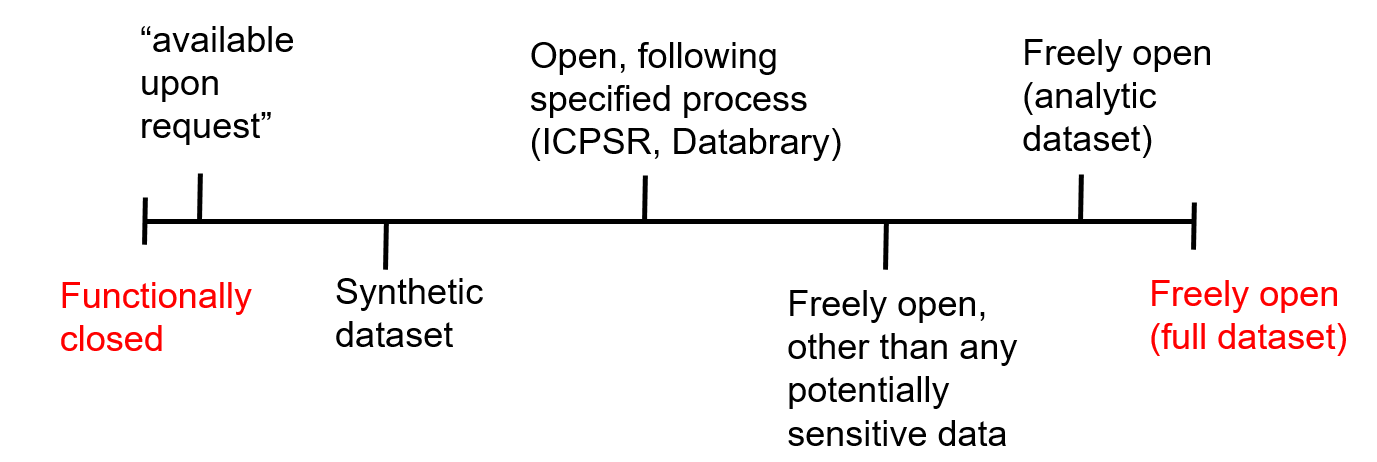
\includegraphics[width=\linewidth]{media/image1.png}

    \caption{A continuum of data sharing}

    \label{fig:rId10}

  \end{fullwidth}

\end{figure}




\begin{itemize}
  \item \textbf{Freely open (full dataset)}\\
        This is the situation I described previously: the full dataset is publicly posted and available for download and reuse. I have no data to support this claim, but I believe strongly that this is what people have in mind when they argue against data sharing.

















  \item  \textbf{Freely open (analytic dataset)}\\
        An argument that I hear frequently from people is that they would be ok with making their data available, but they are not yet done with it. That is, they have plans for further analyses that could lead to publication, so they do not want someone else to publish their ideas. This is a totally reasonable concern and comes up frequently in the context of large datasets. That said, I suspect that we all vastly overestimate the degree to which we are “not yet done” with our datasets. Speaking for myself, I have had many plans for analyzing data that never came to fruition. More to the point, this concern seems to stem from the belief that the full dataset needs to be shared. Alternatively, authors could share only the data used for the analyses reported in the paper. It is extremely unlikely that a research team would have further plans to publish with the exact same data (at least, I hope so), but making the analytic data available would be useful for error detection or other researchers interested in fitting alternative models to the same data. The latter can even generate an additional publication, with the advent of the Verification Report format \parencites{Chambers2020}. If there are no privacy or ethical concerns, then there is little reason for authors to \emph{not} do this.







  \item \textbf{Freely open, other than sensitive data}\\
        Of course, oftentimes there \emph{are} privacy and ethical concerns with making data available. In this case, an option that can be paired with making the full dataset or analytic dataset available is to not share any of the sensitive variables but make all other data available. For example, if researchers are concerned that including demographics could lead to participant re-identification—which is a real risk for minority participants—then those data could be held back, with a specified process outlined for how they could be obtained and under what conditions (see next).







  \item \textbf{Open following a specified process}\\
        Indeed, sometimes the data simply cannot be made openly available for a variety of reasons. We can now make an important distinction between freely and publicly open data, and data that are openly available only following a specified process. This process could involve an application, which might require researchers to specify how they will store the data and for what purpose they will use it. Researchers can specify, in advance, the conditions under which the data will be shared. This is a suitable option for when the data are potentially identifiable, include sensitive information, or where the consent form may not permit public sharing or certain types of analyses. This option also addresses a concern that arises in discussions of diversity and open science, that sharing data could lead to exploitation of marginalized research participants, as the terms of use of the data can be set by the research team to prevent such a thing. The good news is that researchers do not need to develop this process themselves. The \href{https://www.icpsr.umich.edu/web/pages/}{Inter-university Consortium for Political and Social Research} (ICPSR) has long provided this service. There are also discipline-specific protected repositories, such as \href{https://nyu.databrary.org/}{Databrary} \parencites{Gilmore2016} for developmental research and \href{https://ldbase.org/}{LDbase }\parencites{Hart2020} for educational and developmental research. This option will also typically be a strong fit for qualitative data which, more often than not, will contain identifying information. In addition to the previously named repositories, the \href{https://qdr.syr.edu/}{Qualitative Data Repository} was developed for precisely this purpose.







  \item \textbf{Synthetic dataset}
        \\ Creating a specified process for data sharing is a great way to share data, but it is also time-consuming to set up and manage requests (although I would say a worthy investment of resources). \textcite{Quintana2020} developed an alternative option, developing the R package \emph{synthpop}, which generates simulated data that reproduces various statistical properties of the original dataset while preserving confidentiality of the data. This simulated file is shared in lieu of the actual data.







  \item  \textbf{“Data available upon request}\\
        It is now well-documented that statements of “data available upon request,” which are commonly found in published articles, effectively mean that the data are not available at all \parencites{Gabelica2022}{Miyakawa2020}{Wicherts2006}. Accordingly, researchers should not use these statements, and journals should not allow them, as markers of data sharing.







  \item \textbf{Functionally closed}\\
        Unfortunately, this is the state of much of the research data in psychology, and there is little justification for it. I say “little” justification because there are of course some situations in which the data are so sensitive that they need to be heavily restricted (e.g., some genetic data) or an institutional ethics board has taken a hard line, but these situations are the exception rather than the rule. Sometimes data are functionally closed even \emph{within} a research team. If you are part of a project, and the data are not available for your inspection, absent \emph{compelling} rationale, you should be very concerned.


\end{itemize}





All of the above, with the exception of “data available upon request” and functionally closed, are perfectly acceptable forms of data sharing for different data situations. Readers are encouraged to embrace the maxim, “as open as possible, as closed as necessary,” and seek to make their data FAIR (Findable, Accessible, Interoperable, and Reusable; Wilkinson et al., 2016). Data are too complex and varied to have a one-size-fits-all approach, and I tried to highlight some of the options along the continuum of fully open to fully closed. I urge you to be wary of criticisms about data sharing that do not acknowledge these complexities—or even better, I urge you to actively push back on them, because if they present a binary of extremes, they are simply presenting false information. This is not acceptable.







\section{Myth \#3: Preregistration is only for experimental designs}







I often think about a parallel universe in which the replication crisis did not start in social psychology, but in a different area like developmental or clinical psychology. In many ways, it is unfortunate that social psychology was the origin, because it is one of the most methodologically narrow subfields in psychology. Now, some of you will take issue with that statement and ask for empirical evidence, but plenty of social psychologists have discussed the fact that simple lab experiments dominate the field \parencites{Baumeister2007}{Cialdini2009}{Rozin2001}. Accordingly, the focus of the initial reforms was on the kinds of issues that come up in lab experiments. That meant that we thought about reforms starting with the simplest case, and then had to layer the complexity on top of it. That has certainly been the case with preregistration.







Preregistration involves specifying the research questions, hypotheses, methods, and analyses \emph{before} conducting a study, via a time-stamped and unalterable repository \parencites{Nosek2018}. There are quite a lot of claims about why we should be skeptical about preregistration \parencites{MacEachern2019}{McDermott2022}{Pham2021}{Szollosi2020}. These include that it will stifle creativity, that it devalues exploratory work, that it does not allow you to make mistakes or change your mind, that it is unnecessary if you have strong theory, that is it redundant with the ethics application, that it is too bureaucratic, and that it is not appropriate for \_\_\_\_\_\_\_\_ work (fill in the blank with qualitative, longitudinal, secondary data, etc.). These are all false claims based on limited understanding of what preregistration is and why we should do it\footnote{ The one possible exception is the claim that preregistration is unnecessary if you have strong theory \parencite{Szollosi2020}. This could be the case for some areas of psychology, but the vast majority of “theory” in psychology is quite weak, and certainly does not constrain decision-making. Rather, in most cases it makes it worse \parencites{LeBel2011}. Moreover, if you follow my subsequent arguments, even if a study does have a strong formal theory that guides it, there are benefits to specifying the study plans in advance. }, but my focus here is on the last one, that it is not appropriate for certain types of work.







One of the challenges of understanding preregistration—and the criticisms of it—are that there are different rationales for why researchers should do it. These include clearly distinguishing between what decisions were made prior to seeing the data (“confirmatory” analyses) from what decisions were made after seeing the data (“exploratory” analyses), and preventing the latter as being framed as the former in a research report \parencites{Wagenmakers2012}; reducing the prevalence of undisclosed data-dependent decision-making \parencites[i.e., \emph{p}-hacking, questionable research practices, researcher degrees of freedom;][]{Srivastava2018}; evaluating the severity of a test \parencites{Lakens2019}; and serving as formal documentation of the study design and analysis plan \parencites{Haven2019}.







Of course, these rationales are not mutually exclusive, and can all work together. Indeed, for me it is the final rationale—to serve as formal documentation of the design and analysis plan—that is the most functional way to think about preregistration and subsumes all of the other rationales. Thinking of it in this way has rather massive implications for the practice. If you think of preregistration as formal specification of the study design, then \emph{it is clearly applicable to any type of research}. There is no form of research in which absolutely no plans or intentions exist prior to data collection or analysis. That is just not possible. Even a radically exploratory qualitative study involves the specification of a research question, a plan for recruiting participants into the study, some idea of what questions will be asked or how observations will be made, and ideally some plans for how the responses will be analyzed. All of this can be specified ahead of time, and to great benefit to the project.







Some might counter this argument by stating that preregistration is not necessary to achieve the aforementioned goals. Rather, researchers can maintain a rigorous and detailed “lab notebook” approach in which they include all details of a project prior to implementation \parencites[see][for a discussion of this approach in relation to preregistration]{Cruwell2019}. I think that this is technically true, but also there is something quite different about posting the plans to a permanent, unalterable, and public repository. Doing so makes the plans feel somehow more real, and it is also a clear step in the project development phase, marking the transition to project execution. After working with many students on preregistrations over many years, I can assure you that they hold a very different meaning from if they were only kept internally.







Indeed, a major reason why I am so keen on preregistration is that I have witnessed the benefits time and again when working with students. I assure you that I am quite averse to anything that increases the bureaucratic nature of our work. What preregistration does, more than anything, is \emph{make you think} about what you are doing. If you have to specify your plans in advance, then you have to think about \emph{why} you are doing what you plan to do and \emph{how} you plan to do it. These are questions that are relevant for \emph{all} types of research. Since we started preregistering the work in my research group, I have had much more challenging and generative discussions with students about conceptualization, study design, and data analysis.







That is not to say that preregistration can be implemented with the same ease across study designs. I have experience with many different types of designs, and so have developed a continuum (once again) of difficulty with the practice (\emph{Figure 2}). Difficulty here corresponds to the quantity of details and degrees of uncertainty involved in the preregistration process. At the far end of most difficult, we have longitudinal designs, meta-analyses, and most qualitative designs. At the far end of least difficult, we have simple experiments and exploratory studies. Somewhere in the middle falls observational work and projects using secondary data. This continuum is not meant to be taken as a formal pronouncement of the relative difficulty of preregistering these specific designs that is applicable to all situations. Rather, it is based on my own experience using all of these designs, and more specifically my experience preregistering these designs. All study designs can be preregistered, but the details and difficulty will vary. The value, as far as I am concerned, is high throughout all situations.



\begin{figure}
  \begin{fullwidth}
    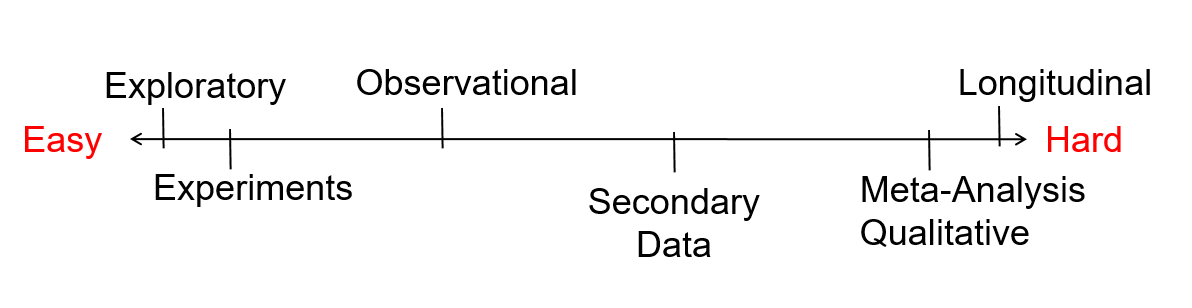
\includegraphics[width=\linewidth]{media/image2.png}

    \caption{Another continuum, this time of preregistration difficulty}

    \label{fig:rId15}

  \end{fullwidth}
\end{figure}



% \subsection{\emph{Figure 2. . }}







Thus, any statements about, “preregistration is not appropriate for \_\_\_\_\_\_\_\_” are simply wrong. Preregistration can be used for any study design, although of course it will look different for different designs. Once again, we should actively reject any arguments—those that are both for and against open science practices—that take a one-size-fits-all approach. This may have been the case in the early days of advocacy for the practice, but our collective thinking has evolved on the issue, and the associated criticisms must be aware of that progress. There are some very smart and industrious people working on how to handle preregistration across the variability in study designs. For example, there are now templates and guides for how to preregister qualitative studies \parencites{Haven2019}, secondary data \parencites{Weston2019}, and meta-analyses \parencites{Moreau2022}, among many others. These folks have embraced the attitude I have repeated several times, that criticisms should not end a conversation, but serve as a launching point to continue the conversation and generate solutions.







Importantly, preregistration is \emph{not} about getting everything right or perfect. We are fallible humans, and mostly mediocre scientists, so we \emph{will} make mistakes. Deviations from a preregistration plan are perfectly acceptable so long as they are transparently reported \parencites{Willroth2023}. At that point, it is up to the reader to determine how the deviation impacts the credibility of the study. On that note, I want to stress that just because a study is preregistered, that does not mean that it is a quality study. I have seen plenty of bad preregistered studies, including those that have undisclosed deviations \parencites[see][]{Claesen2021}. It does, however, allow readers greater information about how the study was planned relative to how it was reported, and thus facilitates stronger interpretations of the stated claims.







\section{Conclusion}







Thirteen years since the start of the replication crisis in psychology, along with the many efforts to identify problems in other fields, tells me that we should all know and admit that we have problems with how we do our science. As I stated from the outset, I very intentionally use “we” because it is true for all of us. None of us are immune, within psychology for sure, but also across the sciences. To paraphrase Simine Vazire, a prominent leader in the scientific reform movement, if you don't think your field has a problem, that's probably because you haven't looked.\footnote{(Simine is not sure that she ever said this but agrees that it sounds like something she would have said; personal communication Dec 14, 2021)}







At this point, given all that we know, it is irresponsible to be an active psychological scientist and to not be informed about the problems that have been unearthed via the replication crisis, and the solutions that have been proposed as part of the open science movement. The keyword is \emph{informed}. Opinions are cheap and plentiful, and it is easy to have a negative reaction about a new practice that is quite different from what you have been accustomed to. Such reactions, however, are often based on uninformed, surface understandings of the issues, rather than careful study and consideration of the details. To reiterate, criticism is good and needed, and it is far from clear that certain open science practices are an unqualified good or benefit to the quality of research. But uninformed criticism and criticism that retreads previously resolved issues is not helpful. Here, I highlighted three recurring debates—about diversity and open science, data sharing, and preregistration—that I argue have been based on insufficient information. As active scientists in the field, it is our responsibility to reject and correct such false claims if we are to have any hope for progress.






\printbibliography



\end{document}